\newpage
\lecture{12}{Интеграл Лебега для неотрицательных функций.}

\begin{theorem}
    Пусть $\forall n\in \N$ функция $f_n:\: X\to\oR$ измерима относительно $\CE$. Тогда
    функции
    \begin{align*}
         & f(x)=\sup_{n\in\N} f_n(x),\quad g(x)=\inf_{n\in\N}f_n(x), \\
         & F(x)=\overline{\lim_{n\to\infty}}f_n(x),\quad
        G(x)=\lim_{\overline{n\to\infty}}f_n(x)
    \end{align*}
    измеримы относительно $\CE$.

    \begin{proof}

        Докажем для функции $f$. Понятно, что \[
            f(x)>c\Rightarrow\exists n:\: f_n(x)>c.
        \] Поэтому, \[
            \{x:\: f(x)>c\}=\bigcup_{n=1}^{\infty}\{x:\: f_n(x)>c\}\in\CE.
        \]

        Инфинум легко сводится к супремуму: \[
            \inf_{n\in\N} f_n(x)=-\sup_{n\in\N}(-f_n(x)).
        \]

        Далее разберемся с верхним пределом: \[
            \overline{\lim_{n\to\infty}}f_n(x)=\lim_{n\to\infty}\underbrace{\sup_{k\geqslant n}f_k(x)}_{\varphi_n(x)}.
        \]
        В силу доказанного имеем $\varphi_n$~--- измеримы. Осталось заметить, что \[
            \varphi_{n+1}(x)\leqslant\varphi_n(x).
        \]
        Благодаря данному неравенству можно записать \[
            \lim_{n\to\infty}\sup_{k\geqslant n}f_k(x)=\inf_{n\in\N}\sup_{k\geqslant n} f_k(x)\text{~--- измеримо.}
        \]
        С нижним пределом аналогично.

    \end{proof}
\end{theorem}

\begin{next0}
    Если $f_n$ измерима $\forall n\in\N$ и $f(x)=\lim\limits_{n\to\infty}f_n(x)$, то $f$~--- измерима (относительно $\CE$).

    В самом деле, в данном случае $\lim\limits_{n\to\infty}f_n(x)=\overline{\lim\limits_{n\to\infty}} f_n(x)$.
\end{next0}

\subsection{Простые функции.}

\begin{definition}
    Функция $s:\: X\to\R$ называется \mdef{простой}, если ее множество значений конечно, то есть
    \begin{gather*}
        \exists n\in\N\quad \exists \{a_i\}_{i=1}^n\subset \R:\quad \exists \{A_i\}_{i=1}^n\subset X:\quad A_i\cap A_j=\varnothing\ (i\neq j):\quad
        X = \bigsqcup_{i=1}^nA_i:\\
        s(x)=\sum_{i=1}^n a_{i}1_{A_i}(x),\quad \forall x\in X.
    \end{gather*}
\end{definition}

\begin{remark}
    По определению простые функции не принимает бесконечных значений. Кроме того,
    простая функция $s$ измерима относительно $\CE$ тогда и только тогда, когда $A_i\in\CE\ \forall i\in\overline{1,n}$,
    так как $A_i=s^{-1}(\{a_i\})$.
\end{remark}

\begin{claim}
    Пусть $f:\: X\to[0,\,+\infty]$ измерима относительно $\CE$. Тогда существует последовательность
    $\{s_n\}_{n=1}^{\infty}$ простых измеримых относительно $\CE$ функций таких, что
    \begin{enumerate}
        \item $\forall x\in X\quad 0\leqslant s_n(x)\leqslant s_{n+1}(x)\leqslant f(x)\quad\forall n\in\N$.
        \item $\forall x\in X\quad \lim_{n\to\infty} s_n(x)=f(x)$.
    \end{enumerate}

    \begin{proof}

        Построим последовательность монотонных функций $\varphi_n$ (см. рис. \ref{fig:lect12:stairs}).

        \begin{figure}[!ht]
            \centering
            

\tikzset{every picture/.style={line width=0.75pt}} %set default line width to 0.75pt        

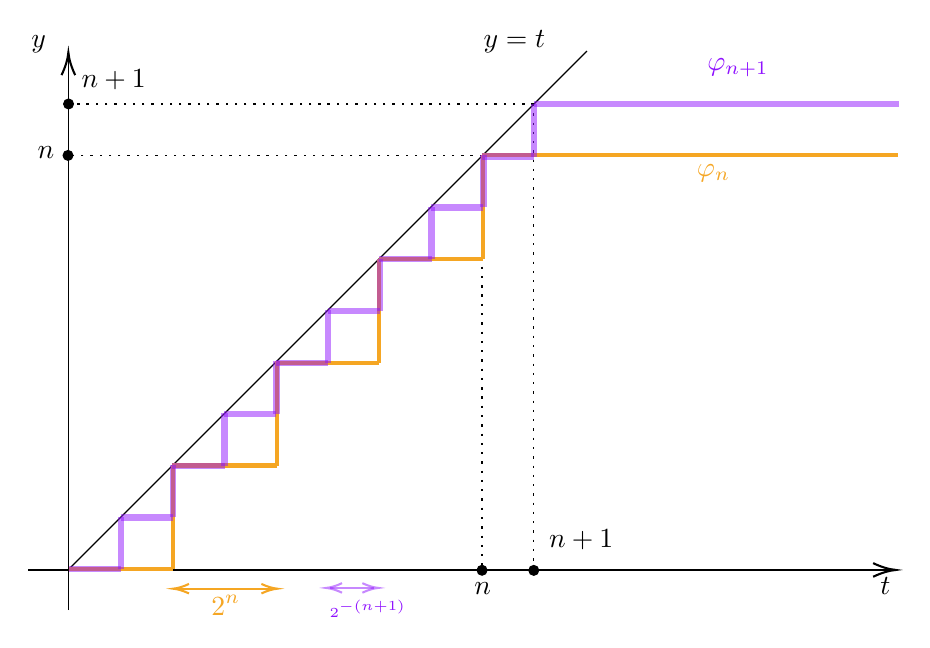
\begin{tikzpicture}[x=0.75pt,y=0.75pt,yscale=-1,xscale=1]
%uncomment if require: \path (0,300); %set diagram left start at 0, and has height of 300

%Straight Lines [id:da5337742975741564] 
\draw    (30.07,280.2) -- (30.07,13.53) ;
\draw [shift={(30.07,11.53)}, rotate = 450] [color={rgb, 255:red, 0; green, 0; blue, 0 }  ][line width=0.75]    (10.93,-3.29) .. controls (6.95,-1.4) and (3.31,-0.3) .. (0,0) .. controls (3.31,0.3) and (6.95,1.4) .. (10.93,3.29)   ;
%Straight Lines [id:da26331508201292997] 
\draw    (10.73,260.87) -- (426.73,260.87) ;
\draw [shift={(428.73,260.87)}, rotate = 180] [color={rgb, 255:red, 0; green, 0; blue, 0 }  ][line width=0.75]    (10.93,-3.29) .. controls (6.95,-1.4) and (3.31,-0.3) .. (0,0) .. controls (3.31,0.3) and (6.95,1.4) .. (10.93,3.29)   ;
%Straight Lines [id:da6016814356247313] 
\draw    (279.9,10.87) -- (30.2,260.57) ;
%Flowchart: Connector [id:dp021415241327152] 
\draw  [fill={rgb, 255:red, 0; green, 0; blue, 0 }  ,fill opacity=1 ] (227,261.02) .. controls (227,259.71) and (228.06,258.65) .. (229.38,258.65) .. controls (230.69,258.65) and (231.75,259.71) .. (231.75,261.02) .. controls (231.75,262.34) and (230.69,263.4) .. (229.38,263.4) .. controls (228.06,263.4) and (227,262.34) .. (227,261.02) -- cycle ;
%Straight Lines [id:da5441061678178924] 
\draw  [dash pattern={on 0.84pt off 2.51pt}]  (229.38,61.15) -- (229.38,261.02) ;
%Flowchart: Connector [id:dp693120063201633] 
\draw  [fill={rgb, 255:red, 0; green, 0; blue, 0 }  ,fill opacity=1 ] (27.52,61.15) .. controls (27.52,59.84) and (28.59,58.77) .. (29.9,58.77) .. controls (31.21,58.77) and (32.27,59.84) .. (32.27,61.15) .. controls (32.27,62.46) and (31.21,63.52) .. (29.9,63.52) .. controls (28.59,63.52) and (27.52,62.46) .. (27.52,61.15) -- cycle ;
%Straight Lines [id:da13074761363997123] 
\draw  [dash pattern={on 0.84pt off 2.51pt}]  (229.38,61.15) -- (29.9,61.15) ;
%Straight Lines [id:da6589479078737384] 
\draw [color={rgb, 255:red, 245; green, 166; blue, 35 }  ,draw opacity=1 ][line width=1.5]    (229.38,61.15) -- (429.9,61.15) ;
%Straight Lines [id:da058055381216781] 
\draw [color={rgb, 255:red, 245; green, 166; blue, 35 }  ,draw opacity=1 ][line width=1.5]    (30.2,260.57) -- (80.4,260.57) ;
%Straight Lines [id:da10237336143893883] 
\draw [color={rgb, 255:red, 245; green, 166; blue, 35 }  ,draw opacity=1 ][line width=1.5]    (80.4,210.65) -- (80.4,260.57) ;
%Straight Lines [id:da21103966169449184] 
\draw [color={rgb, 255:red, 245; green, 166; blue, 35 }  ,draw opacity=1 ][line width=1.5]    (80.2,210.57) -- (130.4,210.57) ;
%Straight Lines [id:da6580458321431404] 
\draw [color={rgb, 255:red, 245; green, 166; blue, 35 }  ,draw opacity=1 ][line width=1.5]    (130.4,160.65) -- (130.4,210.57) ;
%Straight Lines [id:da3456473306288461] 
\draw [color={rgb, 255:red, 245; green, 166; blue, 35 }  ,draw opacity=1 ][line width=1.5]    (129.7,161.07) -- (179.9,161.07) ;
%Straight Lines [id:da40237767964042104] 
\draw [color={rgb, 255:red, 245; green, 166; blue, 35 }  ,draw opacity=1 ][line width=1.5]    (179.9,111.15) -- (179.9,161.07) ;
%Straight Lines [id:da8271931320134389] 
\draw [color={rgb, 255:red, 245; green, 166; blue, 35 }  ,draw opacity=1 ][line width=1.5]    (179.7,111.07) -- (229.9,111.07) ;
%Straight Lines [id:da862391877928931] 
\draw [color={rgb, 255:red, 245; green, 166; blue, 35 }  ,draw opacity=1 ][line width=1.5]    (229.9,61.15) -- (229.9,111.07) ;
%Straight Lines [id:da46062415120687894] 
\draw  [dash pattern={on 0.84pt off 2.51pt}]  (254.3,36.36) -- (254.3,261.07) ;
%Flowchart: Connector [id:dp650088601486764] 
\draw  [fill={rgb, 255:red, 0; green, 0; blue, 0 }  ,fill opacity=1 ] (251.92,261.07) .. controls (251.92,259.76) and (252.99,258.7) .. (254.3,258.7) .. controls (255.61,258.7) and (256.67,259.76) .. (256.67,261.07) .. controls (256.67,262.39) and (255.61,263.45) .. (254.3,263.45) .. controls (252.99,263.45) and (251.92,262.39) .. (251.92,261.07) -- cycle ;
%Straight Lines [id:da6251241144870054] 
\draw  [dash pattern={on 0.84pt off 2.51pt}]  (254.3,36.36) -- (30.15,36.36) ;
%Straight Lines [id:da18782009430462732] 
\draw [color={rgb, 255:red, 144; green, 19; blue, 254 }  ,draw opacity=0.5 ][line width=2.25]    (30.2,260.57) -- (55.3,260.57) ;
%Straight Lines [id:da8541607634935215] 
\draw [color={rgb, 255:red, 144; green, 19; blue, 254 }  ,draw opacity=0.5 ][line width=2.25]    (55.3,260.57) -- (55.3,235.22) ;
%Straight Lines [id:da3272563656451528] 
\draw [color={rgb, 255:red, 144; green, 19; blue, 254 }  ,draw opacity=0.5 ][line width=2.25]    (55.2,235.57) -- (80.3,235.57) ;
%Straight Lines [id:da21032186159846344] 
\draw [color={rgb, 255:red, 144; green, 19; blue, 254 }  ,draw opacity=0.5 ][line width=2.25]    (80.3,235.57) -- (80.3,210.22) ;
%Straight Lines [id:da9426480315832793] 
\draw [color={rgb, 255:red, 144; green, 19; blue, 254 }  ,draw opacity=0.5 ][line width=2.25]    (80.2,210.7) -- (105.3,210.7) ;
%Straight Lines [id:da05661273715373527] 
\draw [color={rgb, 255:red, 144; green, 19; blue, 254 }  ,draw opacity=0.5 ][line width=2.25]    (105.3,210.7) -- (105.3,185.36) ;
%Straight Lines [id:da7866764321453434] 
\draw [color={rgb, 255:red, 144; green, 19; blue, 254 }  ,draw opacity=0.5 ][line width=2.25]    (105.2,185.7) -- (130.3,185.7) ;
%Straight Lines [id:da3554970752960922] 
\draw [color={rgb, 255:red, 144; green, 19; blue, 254 }  ,draw opacity=0.5 ][line width=2.25]    (130.3,185.7) -- (130.3,160.36) ;
%Straight Lines [id:da3942344679086316] 
\draw [color={rgb, 255:red, 144; green, 19; blue, 254 }  ,draw opacity=0.5 ][line width=2.25]    (129.95,161.2) -- (155.05,161.2) ;
%Straight Lines [id:da8572796464883323] 
\draw [color={rgb, 255:red, 144; green, 19; blue, 254 }  ,draw opacity=0.5 ][line width=2.25]    (155.05,161.2) -- (155.05,135.86) ;
%Straight Lines [id:da8424770125255647] 
\draw [color={rgb, 255:red, 144; green, 19; blue, 254 }  ,draw opacity=0.5 ][line width=2.25]    (154.95,136.2) -- (180.05,136.2) ;
%Straight Lines [id:da6205421173979202] 
\draw [color={rgb, 255:red, 144; green, 19; blue, 254 }  ,draw opacity=0.5 ][line width=2.25]    (180.05,136.2) -- (180.05,110.86) ;
%Straight Lines [id:da014750670588427495] 
\draw [color={rgb, 255:red, 144; green, 19; blue, 254 }  ,draw opacity=0.5 ][line width=2.25]    (179.95,111.2) -- (205.05,111.2) ;
%Straight Lines [id:da35945635521343156] 
\draw [color={rgb, 255:red, 144; green, 19; blue, 254 }  ,draw opacity=0.5 ][line width=2.25]    (205.05,111.2) -- (205.05,85.86) ;
%Straight Lines [id:da38203051595889037] 
\draw [color={rgb, 255:red, 144; green, 19; blue, 254 }  ,draw opacity=0.5 ][line width=2.25]    (204.95,86.2) -- (230.05,86.2) ;
%Straight Lines [id:da49644580617059053] 
\draw [color={rgb, 255:red, 144; green, 19; blue, 254 }  ,draw opacity=0.5 ][line width=2.25]    (230.05,86.2) -- (230.05,60.86) ;
%Straight Lines [id:da8885572822737906] 
\draw [color={rgb, 255:red, 144; green, 19; blue, 254 }  ,draw opacity=0.5 ][line width=2.25]    (229.2,61.7) -- (254.3,61.7) ;
%Straight Lines [id:da08674403402809316] 
\draw [color={rgb, 255:red, 144; green, 19; blue, 254 }  ,draw opacity=0.5 ][line width=2.25]    (254.3,61.7) -- (254.3,36.36) ;
%Straight Lines [id:da7613551830060303] 
\draw [color={rgb, 255:red, 144; green, 19; blue, 254 }  ,draw opacity=0.5 ][line width=2.25]    (254.3,36.36) -- (430.3,36.36) ;
%Straight Lines [id:da6604222876823809] 
\draw [color={rgb, 255:red, 245; green, 166; blue, 35 }  ,draw opacity=1 ][line width=0.75]    (82.53,269.9) -- (128.73,269.9) ;
\draw [shift={(130.73,269.9)}, rotate = 180] [color={rgb, 255:red, 245; green, 166; blue, 35 }  ,draw opacity=1 ][line width=0.75]    (7.65,-2.3) .. controls (4.86,-0.97) and (2.31,-0.21) .. (0,0) .. controls (2.31,0.21) and (4.86,0.98) .. (7.65,2.3)   ;
\draw [shift={(80.53,269.9)}, rotate = 0] [color={rgb, 255:red, 245; green, 166; blue, 35 }  ,draw opacity=1 ][line width=0.75]    (7.65,-2.3) .. controls (4.86,-0.97) and (2.31,-0.21) .. (0,0) .. controls (2.31,0.21) and (4.86,0.98) .. (7.65,2.3)   ;
%Straight Lines [id:da11575785037909592] 
\draw [color={rgb, 255:red, 144; green, 19; blue, 254 }  ,draw opacity=0.5 ][line width=0.75]    (156.28,269.53) -- (177.38,269.53) ;
\draw [shift={(179.38,269.53)}, rotate = 180] [color={rgb, 255:red, 144; green, 19; blue, 254 }  ,draw opacity=0.5 ][line width=0.75]    (7.65,-2.3) .. controls (4.86,-0.97) and (2.31,-0.21) .. (0,0) .. controls (2.31,0.21) and (4.86,0.98) .. (7.65,2.3)   ;
\draw [shift={(154.28,269.53)}, rotate = 0] [color={rgb, 255:red, 144; green, 19; blue, 254 }  ,draw opacity=0.5 ][line width=0.75]    (7.65,-2.3) .. controls (4.86,-0.97) and (2.31,-0.21) .. (0,0) .. controls (2.31,0.21) and (4.86,0.98) .. (7.65,2.3)   ;
%Flowchart: Connector [id:dp04273404202961961] 
\draw  [fill={rgb, 255:red, 0; green, 0; blue, 0 }  ,fill opacity=1 ] (27.78,36.36) .. controls (27.78,35.05) and (28.84,33.98) .. (30.15,33.98) .. controls (31.46,33.98) and (32.53,35.05) .. (32.53,36.36) .. controls (32.53,37.67) and (31.46,38.73) .. (30.15,38.73) .. controls (28.84,38.73) and (27.78,37.67) .. (27.78,36.36) -- cycle ;

% Text Node
\draw (11,2) node [anchor=north west][inner sep=0.75pt]   [align=left] {$\displaystyle y$};
% Text Node
\draw (420,263.33) node [anchor=north west][inner sep=0.75pt]   [align=left] {$\displaystyle t$};
% Text Node
\draw (228.9,-0.13) node [anchor=north west][inner sep=0.75pt]   [align=left] {$\displaystyle y=t$};
% Text Node
\draw (224.38,265.74) node [anchor=north west][inner sep=0.75pt]   [align=left] {$\displaystyle n$};
% Text Node
\draw (13.95,55.86) node [anchor=north west][inner sep=0.75pt]   [align=left] {$\displaystyle n$};
% Text Node
\draw (260.38,240) node [anchor=north west][inner sep=0.75pt]   [align=left] {$\displaystyle n+1$};
% Text Node
\draw (35.13,18.5) node [anchor=north west][inner sep=0.75pt]   [align=left] {$\displaystyle n+1$};
% Text Node
\draw (97.67,271.8) node [anchor=north west][inner sep=0.75pt]   [align=left] {$\displaystyle \textcolor[rgb]{0.96,0.65,0.14}{2^{n}}$};
% Text Node
\draw (154.62,274.32) node [anchor=north west][inner sep=0.75pt]  [font=\tiny] [align=left] {$\displaystyle \textcolor[rgb]{0.56,0.07,1}{2^{-( n+1)}}$};
% Text Node
\draw (331.64,64.15) node [anchor=north west][inner sep=0.75pt]   [align=left] {$\displaystyle \textcolor[rgb]{0.96,0.65,0.14}{\varphi _{n}}$};
% Text Node
\draw (336.64,13.15) node [anchor=north west][inner sep=0.75pt]   [align=left] {$\displaystyle \textcolor[rgb]{0.56,0.07,1}{\varphi _{n+1}}$};


\end{tikzpicture}

            \caption{Построение $\varphi_n$.}
            \label{fig:lect12:stairs}
        \end{figure}

        Возьмем $y=t$, построим <<лестницу>>. Во-первых, $\varphi_n(t)=n,\ \forall t\geqslant n$. При $t<n$ вставим
        лестницу с шагом $2^{-n}$.

        Рассмотрим $s_n(x):=\varphi_n(f(x))$. Во-первых, $\varphi_n$~--- борелевская, поэтому $s_n$~--- измерима.
        Далее, очевидно, $s_n$~--- простая.
        Далее, по построению, \begin{gather*}
            0\leqslant\varphi_n(t)\leqslant\varphi_{n+1}(t)\leqslant t,\\
            \varphi_n(x)\to t\text{ при } x\to\infty.
        \end{gather*}
        Следовательно, $s_n(x)\to f(x)\quad \forall x\in X$.

    \end{proof}
\end{claim}

\subsection{Интеграл Лебега для неотрицательных функций.}

Пусть на измеримом пространстве $(X,\, \CE)$ задана $\sigma$"=аддитивная мера $\mu:\: \CE\to[0,\,+\infty]$.
Пусть $s:\: X\to[0,\, +\infty)$~--- простая измеримая относительно $\CE$ функция.

\begin{definition}
    Интегралом называется следующая сумма:
    \[
        \int sd\mu:=\sum_{a\in s(X)}a\cdot\mu\left(s^{-1}(\{a\})\right).
    \]

    То есть, если $X=\bigsqcup\limits_{i=1}^n A_i$ и $s=\sum\limits_{i=1}^n a_i 1_{A_i}$, то
    \[
        \int sd\mu=\sum_{i=1}^n a_i\cdot\mu(A_i).
    \]

    \begin{remark}
        Если $a_i=0$, а $\mu(A_i)=+\infty$, то $a_i\cdot\mu(A_i)=0$.
    \end{remark}
\end{definition}

Часто рассматривается интеграл по измеримому множеству.
\begin{definition}
    Пусть $A\in\CE$. Тогда интеграл:
    \[
        \int_{A}sd\mu:=\int 1_A\cdot s d\mu=\int\left(0\cdot 1_{A^C}+
        \sum_{i=1}^n a_i\cdot 1_{A\cap A_i}\right)d\mu=\sum_{i=1}^n a_i\mu(A\cap A_i).
    \]

    \begin{remark}
        В частности, \[
            \int_X sd\mu=\int sd\mu,
        \]
        так как $1_X=1$.
    \end{remark}
\end{definition}

\begin{claim}
    Если $s_1$ и $s_2$~--- простые, измеримые относительно $\CE$ функции, то
    \[
        \int(s_1+s_2)d\mu=\int s_1d\mu+\int s_2d\mu.
    \]
\end{claim}

\begin{claim}
    Пусть $s:\: X\to[0,\, +\infty]$~--- простая измеримая относительно $\CE$ функция.
    Тогда \[
        \nu(A)=\int_A sd\mu\text{~--- $\sigma$"=аддитивная мера.}
    \]

    \begin{proof}

        Ранее было доказано, что $\nu$~--- $\sigma$"=аддитивна на $\sigma$"=алгебре $\CE$ тогда и только тогда, когда \[
            \forall\{A_n\}_{n=1}^{\infty}\subset\CE:\quad \nu\left(\bigcup_{k=1}^{n}A_k\right)
            \xrightarrow[n\to\infty]{}\nu\left(\bigcup_{k=1}^{\infty}A_k\right).
        \]
        Пусть $s=\sum\limits_{i=1}^m a_i1_{A_i}.$
        Тогда \[
            \nu\left(\bigcup_{k=1}^n A_k\right)=\sum_{i=1}^m a_i\cdot\mu\left(A_i\cap\bigcup_{k=1}^nA_k\right)
            \xrightarrow[n\to\infty]{}\sum_{i=1}^m a_i\mu\left(A_i\cap\bigcup_{k=1}^{\infty}A_k\right)=
            \nu\left(\bigcup_{k=1}^{\infty}A_k\right).
        \]

    \end{proof}
\end{claim}

\begin{definition}
    Пусть функция $f:\: X\to[0,\, +\infty]$ измерима относительно $\CE$. Тогда \[
        \int fd\mu:=\sup\left\{\int sd\mu\ \middle|\ \begin{array}{l}
            s:\: X\to[0,\, +\infty)\text{~--- простая измеримая,} \\
            s\leqslant f\text{ на всем } X.
        \end{array} \right\}
    \]

    \begin{remark}
        Говорят, что функция $s$, определенная выше, \mdef{подпирает} $f$.
    \end{remark}
\end{definition}

\begin{theorem}[Леви, о монотонной функции]
    Пусть функция $f_n:\: X\to[0,\, +\infty]\ \forall n\in\N$ измерима относительно $\CE$.
    Пусть \[
        f_{n+1}(x)\geqslant f_n(x)\quad \forall x\in X\quad \forall n\in\N,
        \quad f(x)=\lim_{n\to\infty}=\sup_{n\in\N} f_n(x).
    \]
    Тогда \[
        I=\int fd\mu=\lim_{n\to\infty}\underbrace{\int f_nd\mu}_{I_n}.
    \]

    \begin{remark}
        То есть теорема утверждает, что можно переставлять знаки интеграла и предела.
    \end{remark}

    \begin{proof}

        Для начала заметим, что \[
            f_n(x)\leqslant f_{n+1}(x)\leqslant f(x)\quad\forall x\in X\quad \forall n\in\N\quad
            \Rightarrow \quad I_{n}\leqslant I_{n+1}\leqslant I.
        \]

        Пусть $J=\sup_{n}I_n\Rightarrow J\leqslant I$. Осталось доказать, что $J\geqslant I$.

        Для этого достаточно доказать, что для любой простой измеримой относительно $\CE$ функции $s:\: s\leqslant f$
        выполнено \[
            \sup_{n}\int f_nd\mu\geqslant\int sd\mu=\sup_{c\in(0,\, 1)}c\int sd\mu.
        \]

        Следовательно, достаточно доказать для любой фиксированных $s$ и $c\in(0,\, 1)$, что \[
            \sup_{n}\int f_n d\mu\geqslant c\cdot\int sd\mu.
        \]

        Заметим, что если на множестве $A\in\CE$ выполнено $f_n\geqslant cs$, то \[
            \int_A f_nd\mu\geqslant c\int_A sd\mu.
        \]

        Рассмотрим такие множества: $A_n=\{x:\: f_n(x)\geqslant c\cdot s(x)\}$.
        Заметим следующую вещь: \[
            f_n(x)\leqslant f(x),\, f_n(x)\xrightarrow[n\to\infty]{}f(x)\Rightarrow
            \forall x\in X \quad \exists N:\: \forall n>N:\quad f_n(x)\geqslant c\cdot s(x).
        \]
        В самом деле, если $s(x)=0$ это очевидно. Если же $s(x)>0$, то $c\cdot s(x)<s(x)<f(x)$.

        Итак, \[
            \forall x\quad \exists n\in\N\quad x\in A_n\Rightarrow X=\bigcup_{n=1}^{\infty}A_n.
        \]
        Тогда \[
            c\int sd\mu=c\int_X sd\mu=\lim_{n\to\infty} c\int_{\bigcup_{k=1}^n A_k} sd\mu,
        \]
        так как $\nu(A)=\int_A sd\mu$~--- $\sigma$"=аддитивная мера.

        Далее, так как $A_n\subset A_{n+1}\ \forall n\in\N$, получаем \[
            \bigcup_{k=1}^n A_k=A_n\Rightarrow c\int_{\bigcup_{k=1}^n A_k}sd\mu=
            c\int_{A_n}sd\mu\leqslant\int_{A_n}f_nd\mu\leqslant
            \int f_nd\mu\leqslant\sup_{n}\int f_nd\mu.
        \]

    \end{proof}
\end{theorem}

\begin{claim}
    Пусть функции $f,\, g:\: X\to[0,\, +\infty]$ измеримы относительно $\CE$. Тогда \[
        \int(f+g)d\mu=\int fd\mu+\int gd\mu.
    \]

    \begin{proof}

        По доказанному ранее, $\exists\{s_n\}_{n=1}^{\infty},\, \{\varphi_n\}_{n=1}^{\infty}$ простых измеримых относительно $\CE$ функций
        такие, что \begin{gather*}
            s_n(x)\leqslant s_{n+1}(x)\leqslant f(x)\quad \forall x\in X\quad \forall n\in\N,\\
            \varphi_n(x)\leqslant \varphi_{n+1}(x)\leqslant g(x)\quad \forall x\in X\quad \forall n\in\N,\\
            s_n\xrightarrow[n\to\infty]{}f(x),\quad
            \varphi_n\xrightarrow[n\to\infty]{}g(x)\quad \forall x.
        \end{gather*}

        Заметим, что \begin{gather*}
            \int fd\mu=\lim_{n\to\infty}\int s_nd\mu,\\
            \int gd\mu=\lim_{n\to\infty}\int \varphi_nd\mu,
        \end{gather*}
        по теореме о монотонной сходимости.
        Следовательно, \[
            \int fd\mu+\int gd\mu=\lim_{n\to\infty}\left(\int s_nd\mu+\int \varphi_nd\mu\right).
        \]
        Так как $s_n,\, \varphi_n$~--- простые, то \[
            \lim_{n\to\infty}\left(\int s_nd\mu+\int \varphi_nd\mu\right)=
            \lim_{n\to\infty}\int \left(s_n+\varphi_n\right)d\mu.
        \]
        Снова по теореме о монотонной сходимости получаем: \[
            \lim_{n\to\infty}\int \left(s_n+\varphi_n\right)d\mu=
            \int\lim_{n\to\infty}(s_n+\varphi_n)d\mu=
            \int(f+g)d\mu.
        \]

    \end{proof}
\end{claim}